% ============================================
% ===== CAPÍTULO 1: INTRODUCCIÓN =====
% ============================================

\chapter{Introducción}\label{chap:introduccion}

Este capítulo presenta la motivación, el contexto, objetivos y fundamentos del trabajo desarrollado. Se expone la problemática abordada, se definen los objetivos principales y secundarios, y se introduce la tecnología base sobre la cual se asienta el proyecto: el sistema DCD de IONOS Cloud y las APIs Canary.

% ===== SECCIÓN 1.1: OBJETIVOS =====
\section{Motivación}\label{sec:motivacion}
La empresa promotora de este proyecto es Arsys, perteneciente al grupo IONOS, quien identificó
la necesidad tras la creación y posterior ampliación del
\textit{DCD}\footnote{Data Center Designer: plataforma gráfica que permite a los clientes de IONOS diseñar
    y configurar sus propios centros de datos de forma visual.},  Al tratarse de un componente fundamental
para la compañía, se hizo necesario establecer mecanismos de control que garantizaran su correcto
funcionamiento y permitieran su verificación continua.

El subsistema de facturación asociado al \textit{DCD} ---encargado de gestionar los cobros derivados del uso y alquiler de las máquinas físicas que soportan las máquinas virtuales--- constituye un foco crítico de posibles errores. Esta vulnerabilidad se debe, principalmente, a la volatilidad de los tipos de cambio de divisas y a la irregularidad en la duración de los meses, factores que pueden introducir inconsistencias en los cargos calculados.
% ===== SECCIÓN 1.1.1: OBJETIVOS =====
\section{Antecedentes}\label{sec:antecedentes}
Como antecedentes se debe partir desde dos puntos de vista: tanto mis antecedentes como los de la empresa.
\begin{itemize}
    \item \textbf{Mis antecedentes: }Durante mi periodo de prácticas en la empresa, tuve la oportunidad de familiarizarme con el DCD de IONOS y de trabajar con las APIs asociadas a este entorno. Esta experiencia incluyó el desarrollo de pequeños proyectos que me permitieron conocer en profundidad la tecnología subyacente, siendo el más relevante la implementación de un detector de identificadores de recursos de otro servicio de IONOS Cloud a partir de una lista estática.
    \item  \textbf{Antecedentes de la empresa: } Al ser una empresa grande, no es el primer servicio que automatizan, por lo que cuentan con librerías internas y herramientas tanto para automatizar como para hacer que ciertas APIs se ejecuten periódicamente. Por ello, la parte correspondiente a la creación de automatizaciones puede apoyarse en las herramientas de la empresa, lo cual facilitará el trabajo en gran medida.

\end{itemize}
% ===== SECCIÓN 1.2: OBJETIVOS =====
\section{Objetivos}\label{sec:objetivos}

\subsection{Objetivo General}
Se consideró necesario desarrollar e implementar un sistema de gestión de automatización de tests para los sistemas de negocio de IONOS, específicamente enfocado en la validación de procesos de facturación cloud. Siendo el principal objetivo del proyecto comprobar de forma automática el correcto funcionamiento de la facturación del DCD.

\subsection{Objetivos Específicos}

\begin{enumerate}
    \item \textbf{Analizar} el estado actual de los sistemas de facturación y validación en IONOS Cloud.

    \item \textbf{Diseñar} una arquitectura de automatización de tests que permita la validación cruzada entre sistemas.

    \item \textbf{Implementar} una API REST para la ejecución y gestión de tests automatizados.

    \item \textbf{Desarrollar} un sistema de detección temprana de inconsistencias mediante técnicas de validación periódica, esto es, comprobaciones automatizadas ejecutadas en intervalos regulares (diarias, semanales o mensuales) para contrastar los cargos facturados contra el consumo real..

    \item \textbf{Evaluar} la efectividad del sistema propuesto en términos de precisión, rendimiento y reducción de errores.

    \item \textbf{Documentar} el proceso de desarrollo y los resultados obtenidos para su posible replicación o mejora.
\end{enumerate}
% ===== SECCIÓN 1.3: Metodología del Proyecto =====
\section{Metodología del Proyecto}

La metodología que se ha optado por usar, ya que se ha considerado la más adecuada, es una implementación iterativa incremental. La razón para tomar esta decisión es el hecho de que este proyecto es ideal para esta metodología. Esta se basa en la partición del desarrollo en pequeñas fases, permitiendo comprobar en cada iteración que una parte del proyecto ya es funcional y facilitando la realización de ajustes antes de continuar con funcionalidades nuevas.

Para cada iteración se seguirá un proceso estándar:

\begin{itemize}
    \item \textbf{Definición de objetivos:} En esta parte se definen los módulos del proyecto que se quieren completar, las funciones que se desea que funcionen y en concreto las tareas a realizar.
    \item \textbf{Análisis:} Se realizan los análisis técnicos necesarios para completar las tareas planeadas en la Definición de objetivos.
    \item \textbf{Desarrollo:} Se llevan a cabo las implementaciones necesarias para lograr los objetivos.
    \item \textbf{Comprobaciones:} Se hacen test, que pueden ser tanto manuales como automáticos, para comprobar que funcionan correctamente las funciones deseadas, en un contexto ideal se comprueban las funciones de las iteraciones anteriores, para asegurar no haber dañado ninguna funcionalidad anterior.
    \item \textbf{Valoración:} Tras cada iteración, se evalúa si se han cumplido los objetivos y en caso negativo las causas.
\end{itemize}

\vspace{0.25cm}

La metodología adoptada ofrece flexibilidad para adaptarse a cambios en los requisitos, entregas parciales que generan prototipos funcionales para ajustes iterativos, reducción de riesgos mediante identificación temprana de problemas en ciclos cortos, mejora continua de la calidad a través de revisiones periódicas, y control detallado del progreso para una gestión eficiente de recursos. Esto permite un desarrollo incremental y dinámico donde las funcionalidades se implementan progresivamente.


% ===== SECCIÓN 1.3: ¿QUÉ ES EL DCD DE IONOS CLOUD? =====
\section{¿Qué es el Diseñador de Centros de Datos (DCD) de IONOS Cloud?}\label{sec:dcd-ionos}

\subsection{Definición y Propósito}

El \textbf{Data Center Designer (DCD)} de IONOS Cloud es una plataforma gráfica que permite a los clientes de IONOS diseñar y configurar sus propios centros de datos de forma visual. Permite a los clientes:

\begin{itemize}
    \item \textbf{Provisionamiento de recursos}: Servidores virtuales, almacenamiento, redes.
    \item \textbf{Gestión del ciclo de vida}: Creación, modificación y eliminación de recursos.
    \item \textbf{Monitorización}: Supervisión del estado y rendimiento de la infraestructura.
    \item \textbf{Facturación}: Cálculo y generación de cargos basados en consumo.
\end{itemize}

Es muy intuitivo y tiene una interfaz bien desarrollada como se puede observar en la imagen.

\begin{figure}[htb]
    \begin{center}
        \vspace*{0.3in}
        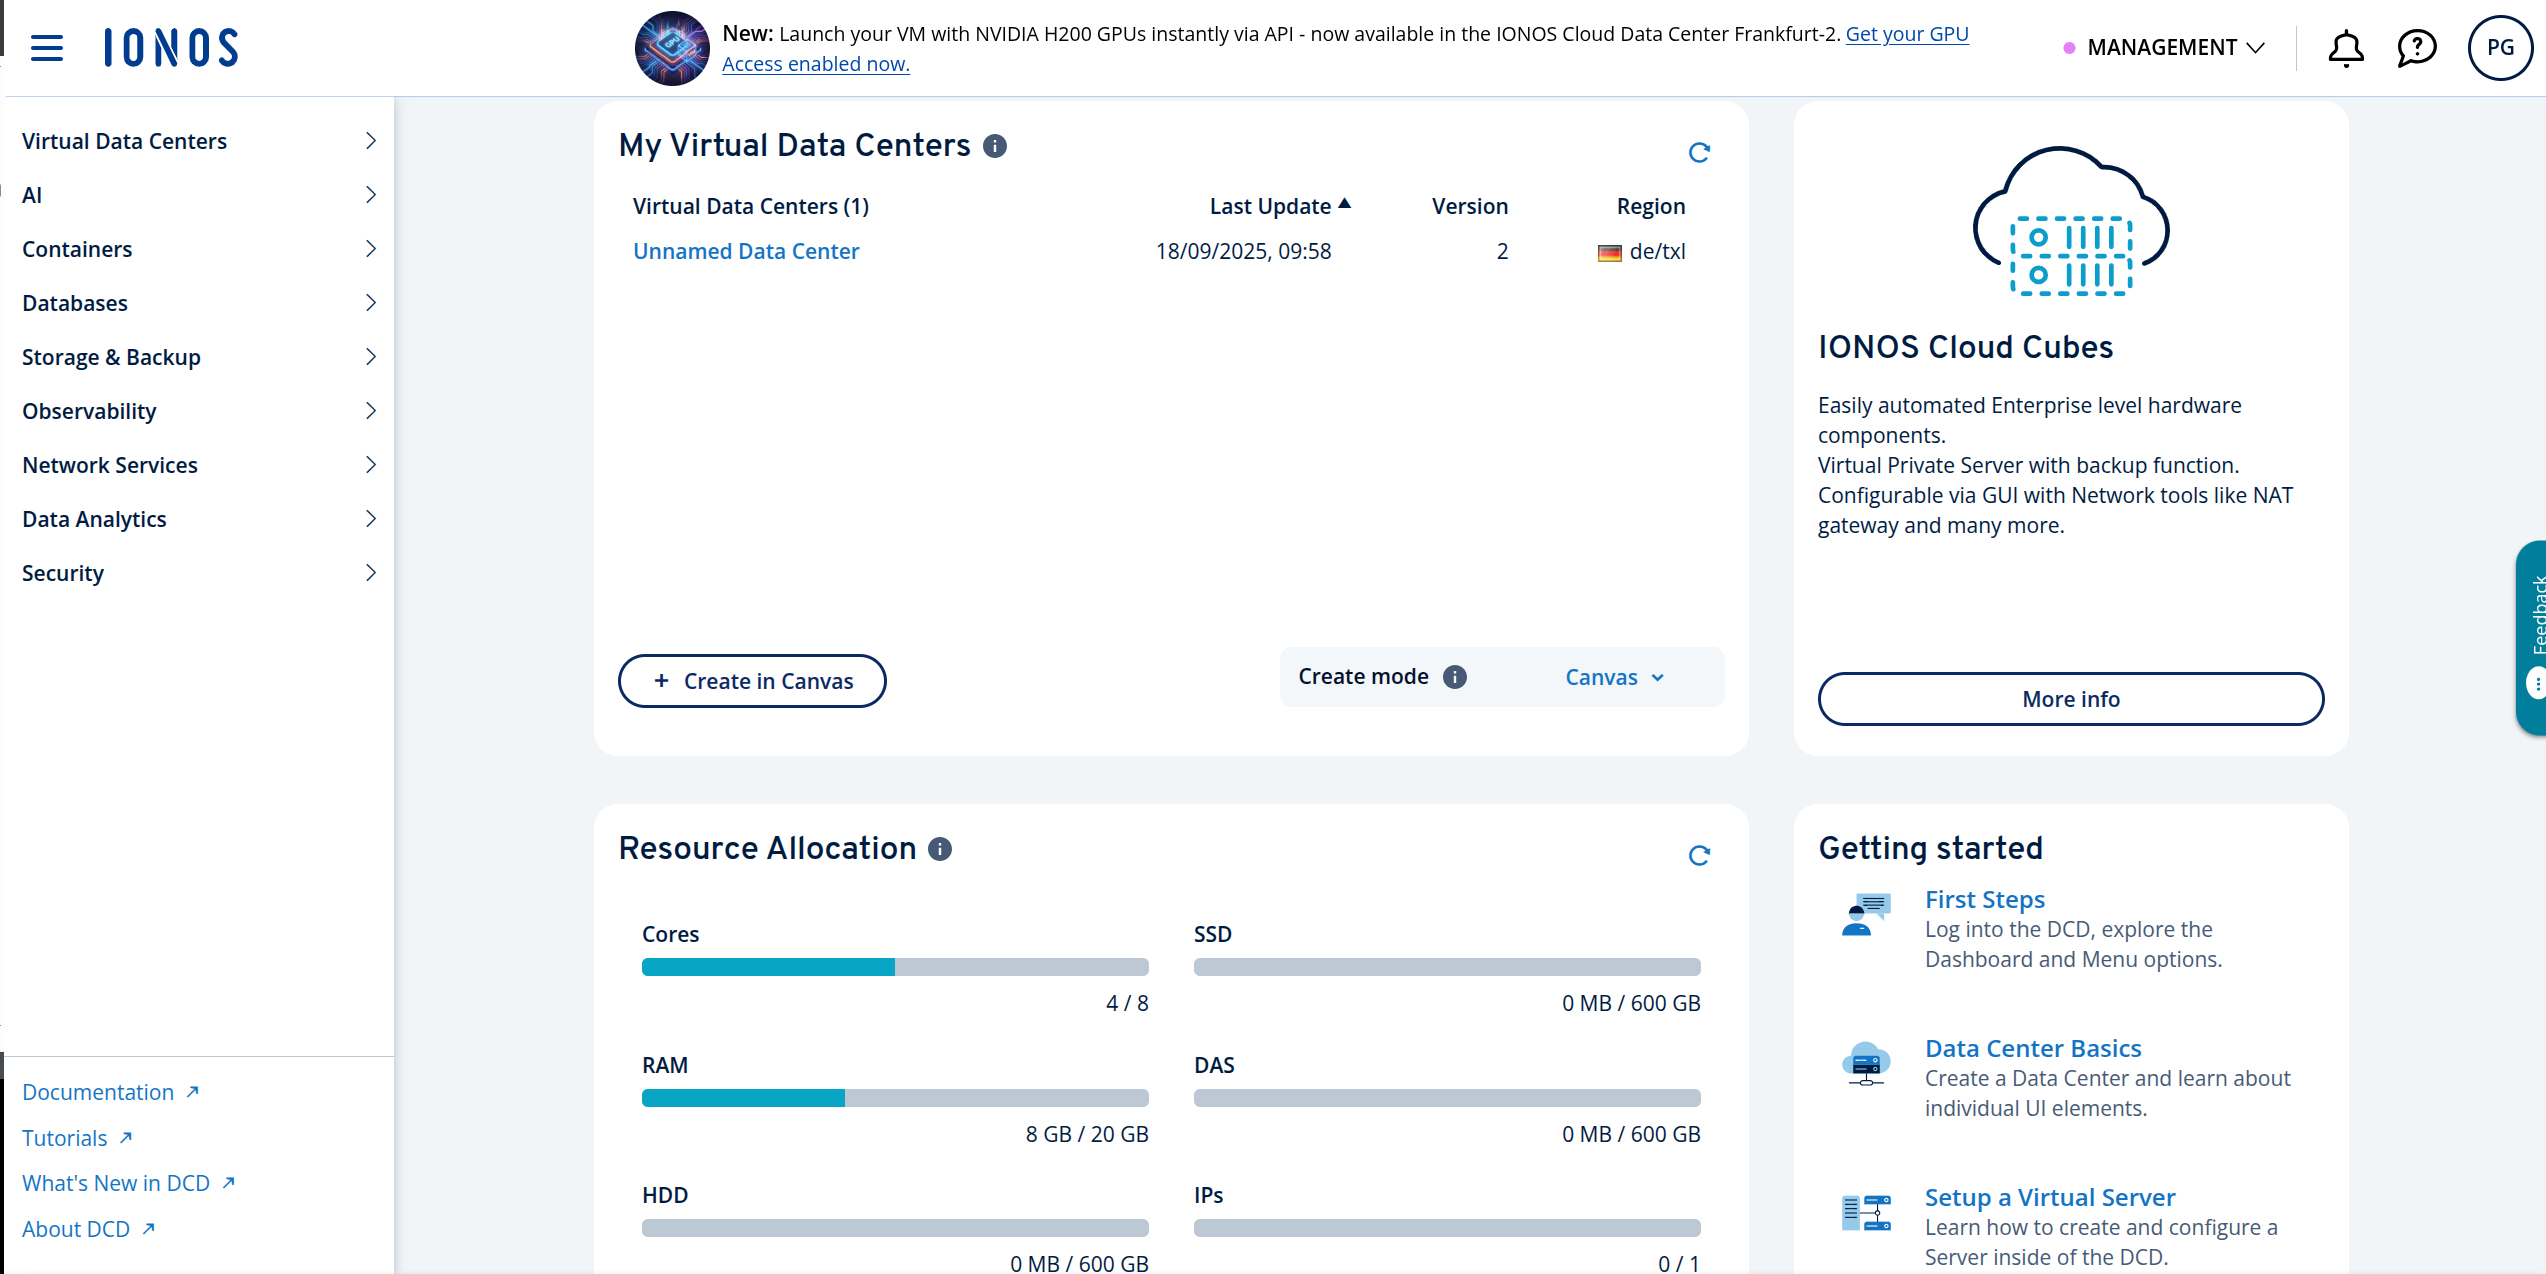
\includegraphics[width=13.5cm]{./imagenes/interfaz-DCD-1.png}
        \caption{Interfaz inicial DCD IONOS Cloud}
    \end{center}
\end{figure}

\newpage


\subsection{Funciones y Herramientas del DCD}

La arquitectura del DCD se compone de múltiples microservicios que interactúan a través de la capa gráfica una vez dentro del diseñador, como se muestra en la imagen.

\vspace{0.25cm}

\begin{figure}[h!]
    \centering
    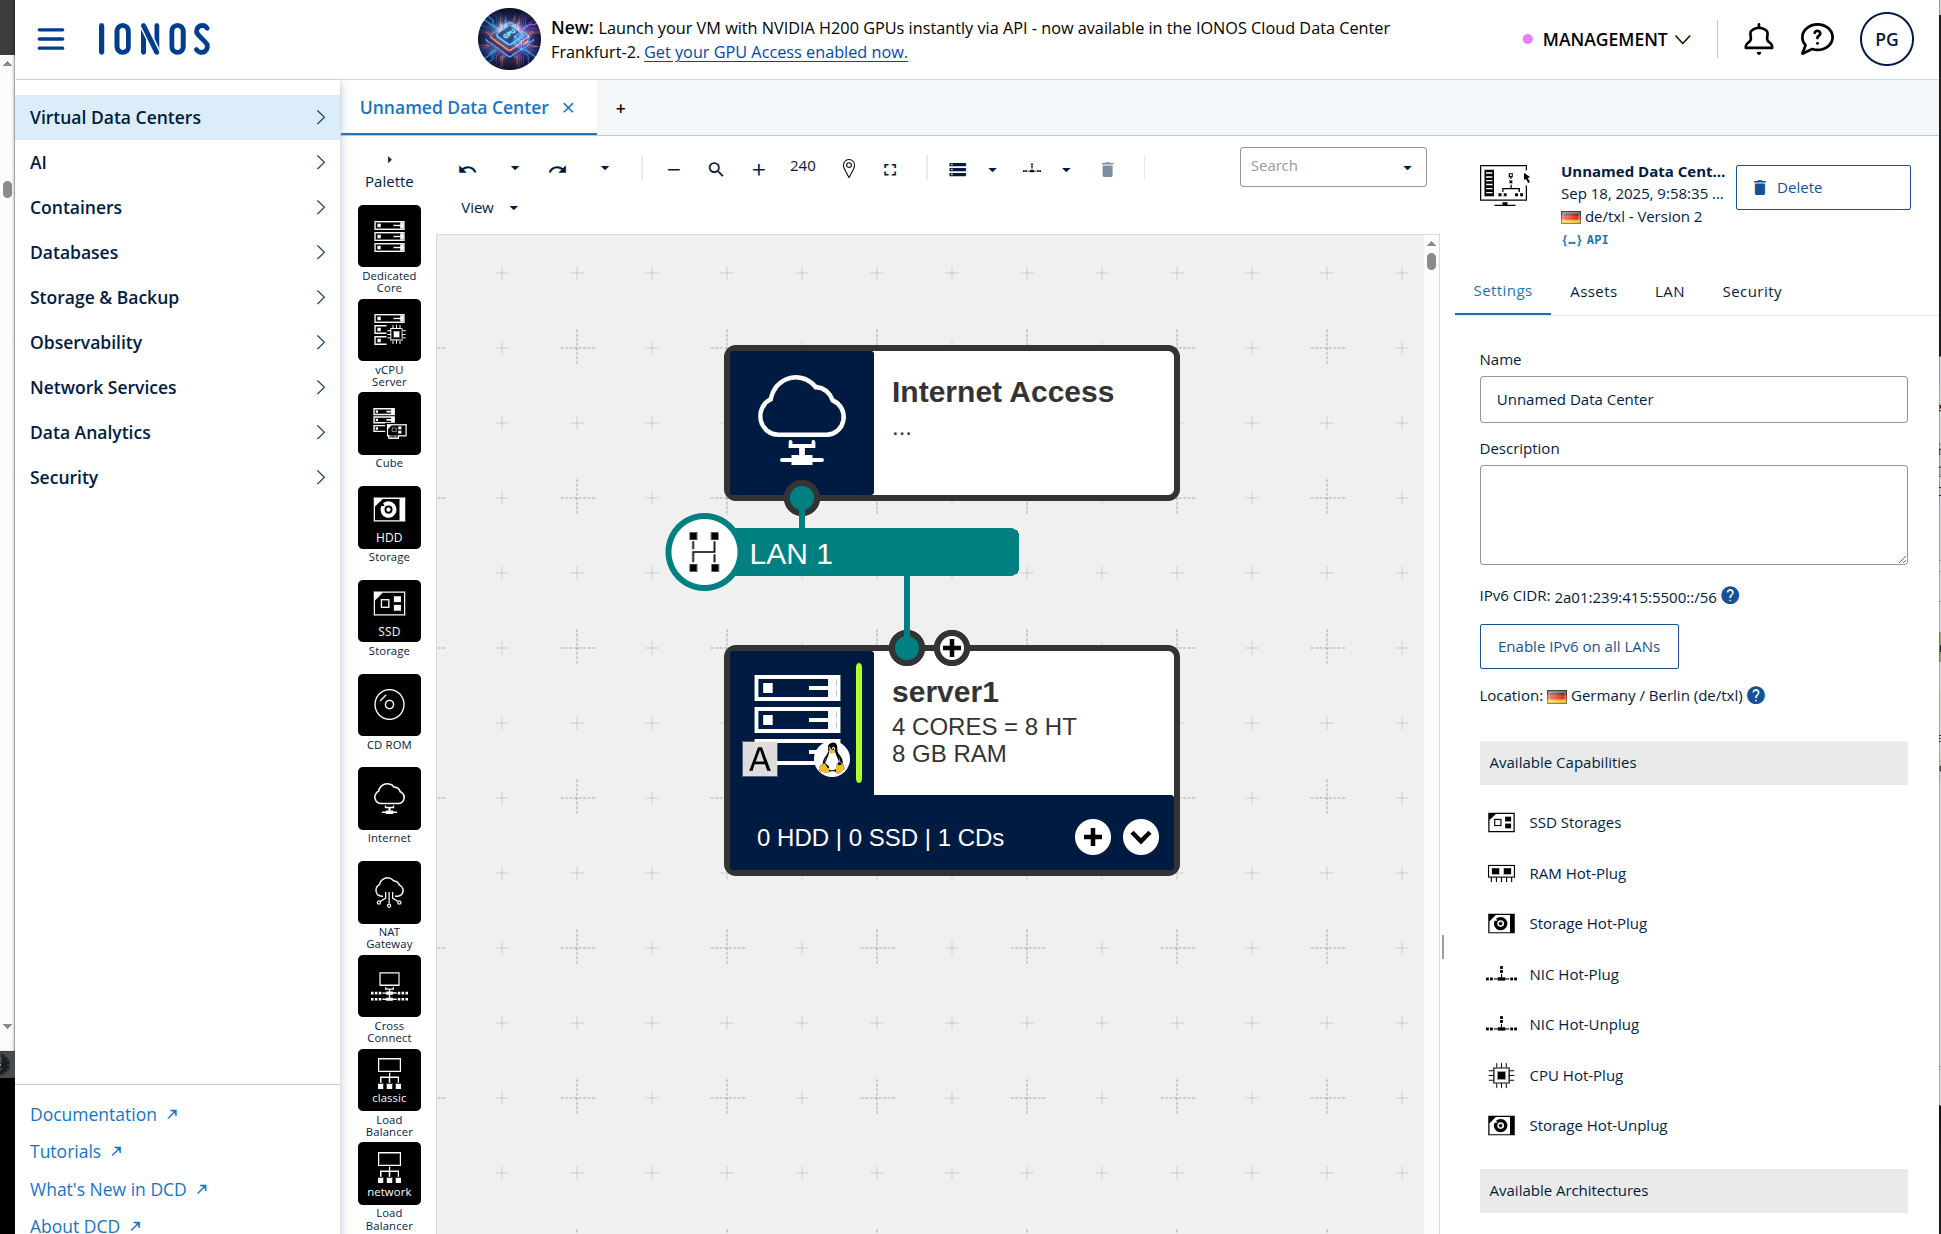
\includegraphics[width=13.5cm]{./imagenes/interfaz-DCD-2.png}
    \caption{Interfaz en Centro de Datos del DCD IONOS Cloud}
    \label{fig:dcd-arquitectura}
\end{figure}

\subsubsection{Herramientas del DCD}

El DCD tiene muchas herramientas y es importante conocerlas para este proyecto, porque para controlar la facturación hay que saber los tipos de elementos que forman el DCD.

\begin{enumerate}
    \item \textbf{Diseñador Gráfico: } Interfaz principal en la que se pueden añadir los recursos principales que se desglosan en el \hyperref[anexo:Lista-de-SKUs]{Anexo 1}.

    \item \textbf{Inteligencia Artificial: } Tiene una herramienta de apoyo de inteligencia artificial de varios modelos; se mide su uso por medio de \textit{tokens}\footnote{Un \textit{token} es una cadena alfanumérica única y secreta generada por un servidor para autenticar y autorizar a un cliente (aplicación, usuario o dispositivo) al realizar solicitudes.}.

    \item \textbf{Contenedores:} es la categoría que agrupa las herramientas para la modernización de aplicaciones (cloud-native). Ofrece dos servicios esenciales y sinérgicos:
          \begin{itemize}
              \item \textbf{Container Registry}: el ``dónde'' guardas tus componentes de software empaquetados (imágenes).
              \item \textbf{Managed Kubernetes}: el ``cómo'' los pones en producción de forma automática, escalable y resistente.
          \end{itemize}

    \item \textbf{Bases de datos: } Conjunto de datos organizado de tal modo que permita obtener con rapidez diversos tipos de información. Hay tanto relacionales como no relacionales, para más información consultar el anexo 1.

    \item \textbf{ Almacenamiento y Copias de Seguridad:} En el \textit{DCD}, Storage y Backup son pilares complementarios de la estrategia de datos, siendo el Almacenamiento donde ``viven'' mis datos ahora mismo y las copias de seguridad la manera de recuperar dicha información. Ofrece cinco servicios:
          \begin{itemize}
              \item \textbf{ IONOS Object Storage: } Almacén masivo para archivos y objetos.
              \item \textbf{ Network File Storage: } Sistema de archivos compartido en red.
              \item \textbf{ Backup Unit Manager: } Herramienta de automatización y gestión de copias de seguridad.
              \item \textbf{ Images y Snapshots: } Captura del estado del sistema para revertir o clonar.
              \item \textbf{ FTP Image Upload: } Importación de plantillas personalizadas de sistemas.
          \end{itemize}
    \item \textbf{Servicios de red: } Define cómo se conectan y comunican todos los recursos, es una de las partes más importantes, desglosándose en varias partes:
          \begin{itemize}
              \item \textbf{Administración de direcciones IP: } gestión centralizada de direcciones IP.
              \item \textbf{Puerta de Enlace VPN: }  Servicio que crea un túnel cifrado y seguro entre tu infraestructura en IONOS Cloud y otro sitio.
              \item \textbf{Red de Distribución de Contenidos: } Una red global de servidores que almacenan en caché copias del contenido est\'atico (im\'agenes, CSS{\textgreater}, JS{\textgreater}, videos) cerca de los usuarios finales.
              \item \textbf{Cloud DNS: } El servicio de resolución de nombres de dominio gestionado por IONOS. Traduce nombres de dominio (www.tuempresa.com) a direcciones IP (185.100.100.10).
          \end{itemize}
    \item \textbf{Seguridad: } Marco de trabajo integrado que aplica múltiples capas de protección:
          \begin{itemize}
              \item \textbf{Manager de llaves SSH:} protege el ``quién''; autenticación fuerte para administradores y automatización.
              \item \textbf{Grupos de Seguridad de Red:} protege el ``qué y dónde''; control estricto del flujo de tráfico entre los recursos.
              \item \textbf{ Gestor de certificados: } protege el ``cómo''; confianza y privacidad para las comunicaciones con los usuarios finales.
          \end{itemize}
\end{enumerate}


% ===== SECCIÓN 1.3: ¿QUÉ ES UNA API CANARY? =====
\section{¿Qué es una API REST y una API Canary?}\label{sec:api-canary}

\subsection{¿Qué es una API REST?}
Una API REST es un intermediario estandarizado que permite que diferentes aplicaciones se comuniquen entre sí mediante el protocolo HTTP.
En el contexto de este proyecto, la API REST desarrollada permite ejecutar y gestionar los tests de validación de facturación, comunicándose
con los servicios de IONOS Cloud para obtener datos de consumo y compararlos con los cargos facturados. Este formato fue requerido por la empresa debido a
su escalabilidad, simplicidad y naturaleza sin estado (cada petición es independiente y autocontenida).
\subsection{Principios REST}
\begin{itemize}
    \item \textbf{Arquitectura Cliente-Servidor: } Clara separación entre el cliente (solicita) y el servidor (responde). En este proyecto, la API de validación actúa como servidor que recibe peticiones y se comunica con los servicios de facturación de IONOS Cloud.
    \item \textbf{Sin Estado: } Cada petición contiene toda la información necesaria. En el proyecto, cada llamada de validación incluye el token de autenticación y los parámetros del test a ejecutar.
    \item \textbf{Cacheable: } Las respuestas pueden almacenarse temporalmente. Esto permite optimizar las consultas repetidas a datos de facturación que no cambian frecuentemente.
    \item \textbf{Interfaz Uniforme: } Todo es un recurso con URI única. La API expone endpoints claros como \texttt{/validation}, \texttt{/products} o \texttt{/utilization}.
    \item \textbf{Sistema en Capas: } El cliente no sabe si está conectado al servidor final o a un intermediario. El sistema puede escalarse añadiendo proxies o balanceadores sin modificar los clientes.

\end{itemize}

\subsection{Concepto y Origen de API Canary}

El término \textbf{``Canary''} proviene de la práctica minera de usar canarios para detectar gases peligrosos. En desarrollo de software, una \textbf{API Canary} se refiere a:

\begin{quote}
    Una implementación de API que se despliega gradualmente a un subconjunto de usuarios o sistemas para detectar posibles problemas antes de que el usuario final lo detecte. El método de funcionamiento es una ejecución periódica con una alarma si falla, la frecuencia de dicha ejecución será dependiente de lo crítico que sea el módulo que controla.
\end{quote}

\subsection{Características Principales}

\begin{table}[h!]
    \centering
    \begin{tabular}{|p{0.3\textwidth}|p{0.6\textwidth}|}
        \hline
        \textbf{Característica}                                                                                                                                                           & \textbf{Descripción}                                       \\
        \hline
        \hline
        \textbf{Despliegue Gradual}                                                                                                                                                       & Se implementa primero a un pequeño porcentaje del tráfico. \\
        \hline
        \textbf{Monitorización Intensiva}                                                                                                                                                 & Se supervisa exhaustivamente en busca de errores.          \\
        \hline
        \textbf{Rollback Automático}                                                                                                                                                      & Si se detectan problemas, se revierte automáticamente.     \\
        \hline
        \textbf{A/B \textit{Testing}\footnote{Es el proceso de evaluar, verificar y validar software u otros sistemas para asegurar que funcionan según lo esperado, detectando errores}} & Permite comparar versiones nuevas vs. antiguas.            \\
        \hline
    \end{tabular}
    \caption{Características de una API Canary}
    \label{tab:api-canary-caracteristicas}
\end{table}

\subsection{Ventajas en Sistemas de Facturación}

La implementación de APIs Canary en sistemas de facturación ofrece:

\begin{itemize}
    \item \textbf{Detección temprana}: Problemas se identifican rápidamente, el tiempo que tarde en detectarse será dependiente de la frecuencia de su ejecución.
    \item \textbf{Reducción de riesgos}: Errores de facturación afectan solo a un subconjunto de clientes. Ya que al detectarse de forma temprana y le afecta a menos clientes.
    \item \textbf{Validación en producción}: Pruebas con datos reales sin comprometer todo el sistema. Ya que se crea un cliente real completo para usar en la API.
    \item \textbf{Mejora continua}: Permite iteraciones rápidas y seguras. Ya que es muy fácil de separar en módulos.
\end{itemize}



\subsection{Flujo de Trabajo Canary}

\begin{figure}[h!]
    \centering
    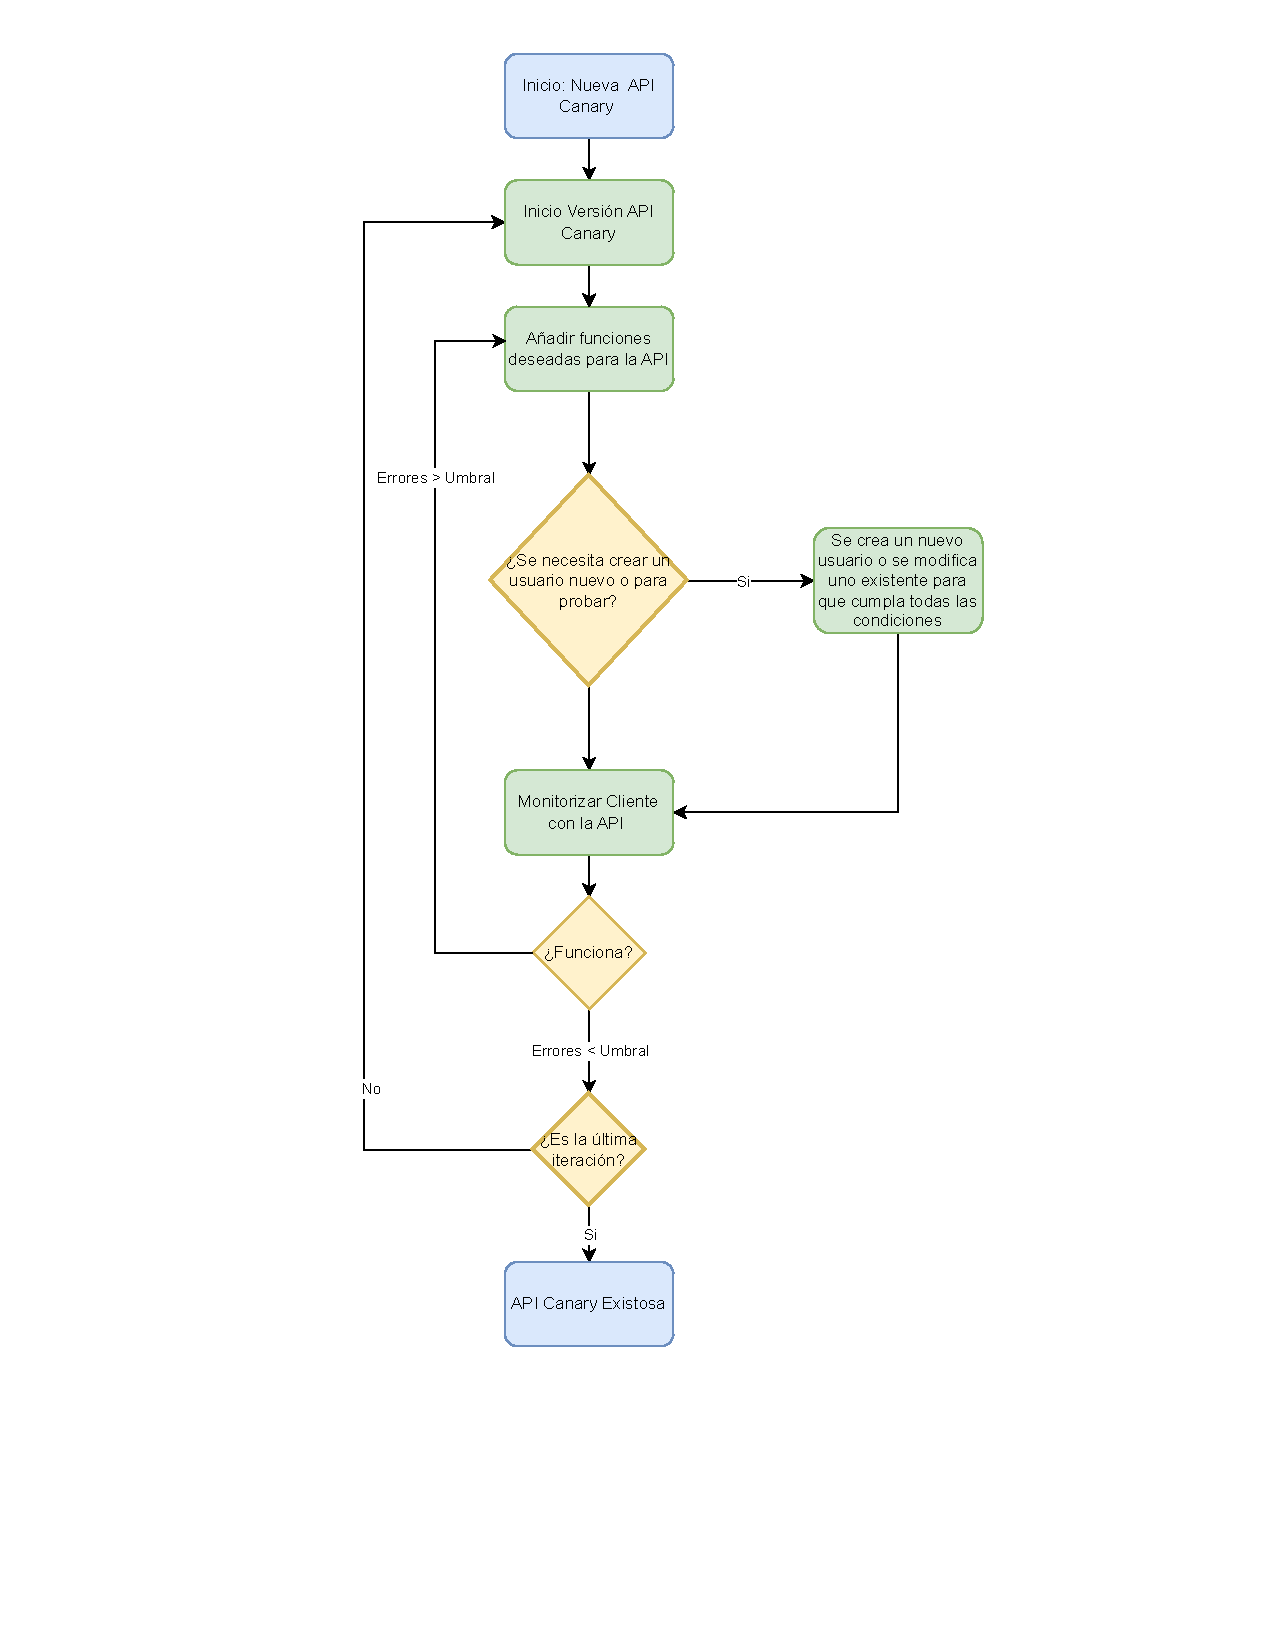
\includegraphics[width=0.9\textwidth]{archivos/flujo_API_Canary.drawio.pdf}
    \caption{Diagrama de flujo del proceso de despliegue Canary para APIs}
    \label{fig:canary-flow}
\end{figure}

\textbf{Descripción del flujo:}
\begin{enumerate}
    \item \textbf{Inicio: Nueva API Canary } - Desarrollo de una nueva  API de validación.

    \item \textbf{Inicio: Nueva Versión API Canary} - Desarrollo de una nueva versión de la API de validación. En la que se inicia la nueva iteración.

    \item \textbf{Inicio: Añadir funciones deseadas} - Se implementan las nuevas funciones deseadas.

    \item \textbf{Comprobación de completitud del usuario de muestra} - Se comprueba que el usuario que se usa para comprobar el correcto funcionamiento de la API tiene todos los recursos necesarios que debe comprobar. En el caso contrario, se modifica para que permita comprobar todas las funciones a comprobar, en su defecto se creará un nuevo perfil para ello.

    \item \textbf{Monitorizar Métricas} - Análisis continuo de errores, latencia y otras métricas clave.

    \item \textbf{Decisión basada en umbrales:}
          \begin{itemize}
              \item \textbf{Si errores < Umbral} → Se pasa a la siguiente fase de la API.
              \item \textbf{Si errores > Umbral} → Rollback automático a versión estable y se revisan las actualizaciones para volver a modificar y lograr hacer funcionales los cambios.
          \end{itemize}

    \item \textbf{API Canary Exitosa} - Tras terminar todas las fases, se integra y entra la fase de automatizarla para que se ejecute periódicamente.
\end{enumerate}

% ===== SECCIÓN 1.4: TECNOLOGIAS Y HERRAMIENTAS =====

\section{Tecnologías y Herramientas Utilizadas}

\noindent Para el desarrollo del sistema de validación de facturación cloud, se ha construido una arquitectura tecnológica robusta que combina herramientas modernas de desarrollo, infraestructura contenerizada y patrones de diseño específicos para el dominio de facturación.

\subsubsection{Stack Tecnológico Principal}

\begin{table}[h!]
    \centering
    \begin{tabular}{|p{0.25\textwidth}|p{0.7\textwidth}|}
        \hline
        \textbf{Categoría}                         & \textbf{Tecnologías}                    \\
        \hline
        \hline
        \textbf{Runtime}                           & Node.js 18+ (LTS)                       \\
        \hline
        \textbf{Lenguaje}                          & JavaScript ES6+ con módulos             \\
        \hline
        \textbf{Framework Web}                     & Express.js con middleware personalizado \\
        \hline
        \textbf{Gestión de Paquetes}               & Yarn 3+ con workspace                   \\
        \hline
        \textbf{Testing}                           & Postman                                 \\
        \hline
        \textbf{Creación de usuarios de muestreo } & DCD de IONOS                            \\
        \hline
        \textbf{Base de Datos Configuración}       & CouchDB para configuración distribuida  \\
        \hline
        \textbf{Control de Versiones}              & GitLab para paquetes internos           \\
        \hline
        \textbf{Editor de Código}                  & Visual Studio Code                      \\
        \hline
        \textbf{Documentación}                     & LaTeX en OverLeaf                       \\
        \hline
        \textbf{Creación de diagramas}             & Draw.io                                 \\
        \hline
        \textbf{Conexión con equipo }              & VPN a red Alemana                       \\
    \end{tabular}
    \caption{Stack tecnológico del proyecto}
    \label{tab:stack-tecnologico}
\end{table}

\subsubsection{Dependencias Clave del Proyecto}

\textbf{Dependencias Internas:}
\begin{itemize}
    \item \texttt{@internal/core} - Framework base con utilidades de inicialización y configuración
    \item \texttt{@internal/dev} - Suite de herramientas para desarrollo y debugging
\end{itemize}

\textbf{Dependencias Externas Críticas:}
\begin{itemize}
    \item \texttt{helmet} - Middleware de seguridad para cabeceras HTTP
    \item \texttt{express} - Framework web minimalista para Node.js
    \item \texttt{couchdb-nano} - Cliente para integración con CouchDB
\end{itemize}

\subsubsection{Arquitectura Modular Implementada}

La arquitectura del sistema se organiza en tres capas principales:

\begin{enumerate}
    \item \textbf{Capa de Infraestructura:}
          \begin{itemize}
              \item CouchDB para gestión de configuración centralizada
          \end{itemize}

    \item \textbf{Capa de Servicios:}
          \begin{itemize}
              \item \texttt{data-api}: Servicio de acceso y transformación de datos
              \item \texttt{invoice-validation}: Motor de validación de facturación
              \item \texttt{utilization}: Procesamiento de métricas de uso
          \end{itemize}

    \item \textbf{Capa de Helpers y Utilidades:}
          \begin{itemize}
              \item Módulo \texttt{schema}: Validación y transformación de datos
              \item Módulo \texttt{actions}: Operaciones comunes del negocio
              \item Módulo \texttt{invoice}: Lógica específica de facturación
          \end{itemize}
\end{enumerate}

\subsubsection{Flujo de Desarrollo y Calidad}

\begin{itemize}
    \item \textbf{Desarrollo Local:} Nodemon para hot-reload durante el desarrollo
    \item \textbf{Calidad de Código:} ESLint con configuración personalizada
    \item \textbf{Control de Cambios:} Hooks pre-commit para validaciones automáticas
    \item \textbf{Integración:} Pipelines CI/CD en GitLab para despliegue continuo
\end{itemize}
